%!TEX root = paper.tex

We next moved on to develop a continuous erosion model that operates on smooth surfaces, in contrast to our previous discrete model that operated on piecewise linear surfaces. Physically this new model represents a surface being worn down gradually, such as a bar of soap in water or an ice cube melting. 

\subsection*{Continuous Surface}

We will start by introducing a set of parametric equations to represent a surface. A parametric representation was chosen over an implicit one, so that we can use spectral methods and the FFT when integrating Equation \ref{eq:erosion-diff-eq}, which we will discuss in detail in Section \ref{sec:numerical-modeling}. 

Let us introduce $s \in [0, 2\pi)$ as our parameter with $s$ increasing counterclockwise along the surface. The coordinates of any point on the surface can be represented at time $t \ge 0$ by two functions $x(t, s), y(t, s)$. Coordinates can be written more compactly as

\[ 
  \bvec{r}(t, s) \coloneqq \paren{x(t, s), y(t, s)}
\]

\textbf{Note:} The reader should keep in mind that derivative operators still apply to each coordinate individually, e.g.

\[
  \frac{\partial \bvec{r}(t, s)}{\partial t} \coloneqq \paren{\frac{\partial x(t, s)}{\partial t}, \frac{\partial y(t, s)}{\partial t}}
\]

To simplify our equations, we introduce the following vector calculus notation

\begin{align*}
  \dot{\bvec{r}}(s)& \coloneqq \frac{\partial \bvec{r}(s)}{ds}\\
  \ddot{\bvec{r}}(s)& \coloneqq \frac{\partial^2 \bvec{r}(s)}{ds^2}
\end{align*}

The equations for the initial shape that we will use in our simulations are shown below and a plot of the shape is shown in Figure \ref{fig:blob-shape} ($T_i$ is the i\textsuperscript{th} Chebyshev polynomial)

\begin{align*}
  x(0, s) = \cos(s) \paren{2 T_0\paren{\frac{s-\pi}{\pi}} + T_2\paren{\frac{s-\pi}{\pi}}}\\
  y(0, s) = \sin(s) \paren{2 T_0\paren{\frac{s-\pi}{\pi}} + T_4(\paren{\frac{s-\pi}{\pi}})}
\end{align*}

\begin{figure}[H]
  \begin{center}
    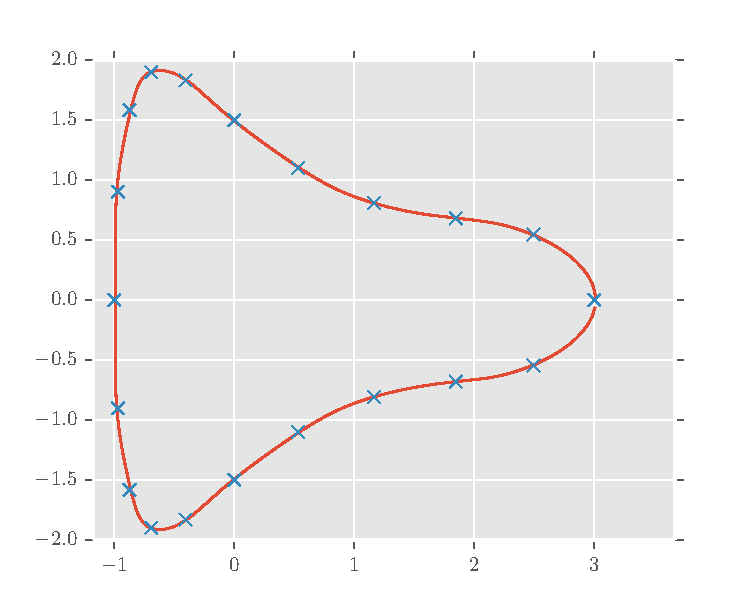
\includegraphics[keepaspectratio, width=4in]{blob_shape.pdf}
  \end{center}
  \vspace{-.2in} % corrects bad spacing
  \caption{\label{fig:blob-shape} Example shape.}
\end{figure}

The method used to represent the shape numerically will be explained in Section \ref{sec:numerical-modeling}, but first we will take a moment to explain the various erosion processes that we will model in this section.

\subsection*{Continuous Erosion Processes}

All of the processes that we will look at in this section, will move points on the surface in the direction of the surface normal, which is defined as

\[
  \hat{n}(\bvec{r}(s)) = (-\dot{y}(s), \dot{x}(s))
\]

We can now model our erosion process with the following differential equation, where $g(\bvec{r}(s))$ is a function specific to the erosion process being modeled.

\begin{equation}
  \label{eq:erosion-diff-eq}
  \frac{\partial \bvec{r}(t, s)}{\partial t} = g(\bvec{r}(s)) \; \hat{n}(\bvec{r}(s))
\end{equation}

\subsubsection*{Smoothing Process}

One of the processes that we will look at is a soap bar being worn down by a person holding it in their hand, which we will call the \textit{Smoothing Process}. In this process, bumps on the object will get worn down quickest, because they are the first parts to come into contact with the person's hand. Technically the furthest protruding bumps will be worn down quickest, but to simplify the problem, we assume that every point on the surface wears down at a rate proportional to the curvature at the point. We will use a signed curvature $\kappa$, so that a bump will have positive curvature, and an indentation will have negative curvature. 

\[
  \kappa(\bvec{r}(s)) = \frac{\dot{\bvec{r}}(s) \times \ddot{\bvec{r}}(s)}{\norm{\dot{\bvec{r}}(s)}^3}
\]

To make bumps erode faster than indentations, we will use the following damping function

\begin{equation}
  g(\bvec{r}(s)) = \tan^{-1}(\beta \, (\kappa(\bvec{r}(s)) - \alpha)) + \frac{\pi}{2}
\end{equation}

For our simulations we chose $\alpha = 1, \; \beta = 5$ so that $g(\bvec{r}(s)) \approx 1$ at the corners on our initial surface. This restriction is not based on the physics of the problem, and was chosen purely for the aesthetic look of the resulting simulation.

\begin{figure}[H]
    \begin{center}
      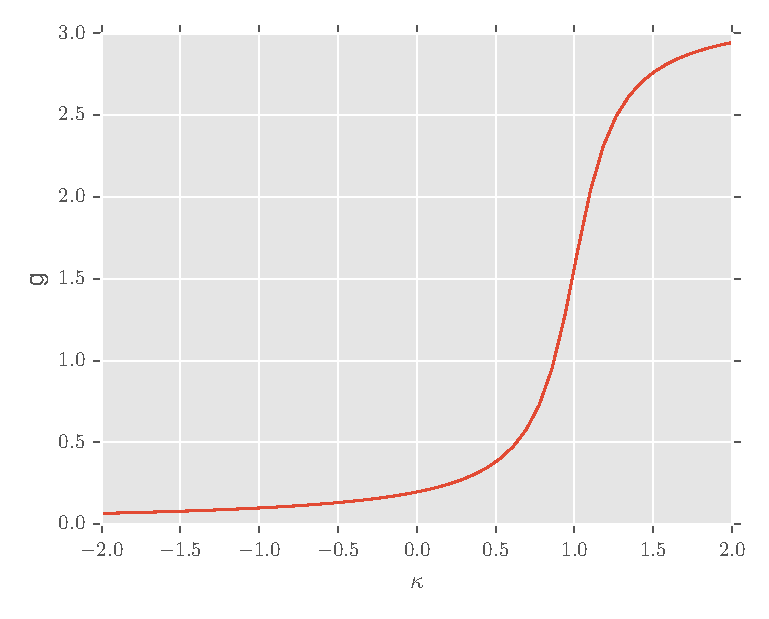
\includegraphics[keepaspectratio, width=4in]{g_1.pdf}
    \end{center}
  \vspace{-.2in} % corrects bad spacing
  \caption{\label{fig:g-1} Plot of $g(\kappa)$ for \textit{Smoothing Process}.}
\end{figure}

\subsubsection*{Bottom Recession Process}

Our second process is an object sitting in a bath of acid, which we will call our \textit{Bottom Recession Process}. In this process, the lowest points (smallest values of $y(s)$) on the surface will erode quickest.

\begin{gather}
  f(s) = \frac{1}{\alpha \, (y(s) - y_{min}) + \beta} - \gamma \notag\\
  g(s) = \begin{cases}
    f(s) \qquad &\text{for} \quad f(s) > 0\\
    0 \qquad &\text{otherwise}
  \end{cases}
\end{gather}

For our simulations we chose $\alpha = 10, \; \beta = \gamma = 0.1$ so that $g(\bvec{r}(s)) \approx 1$ for $y(s) \approx y_{min}$.

\begin{figure}[H]
    \begin{center}
      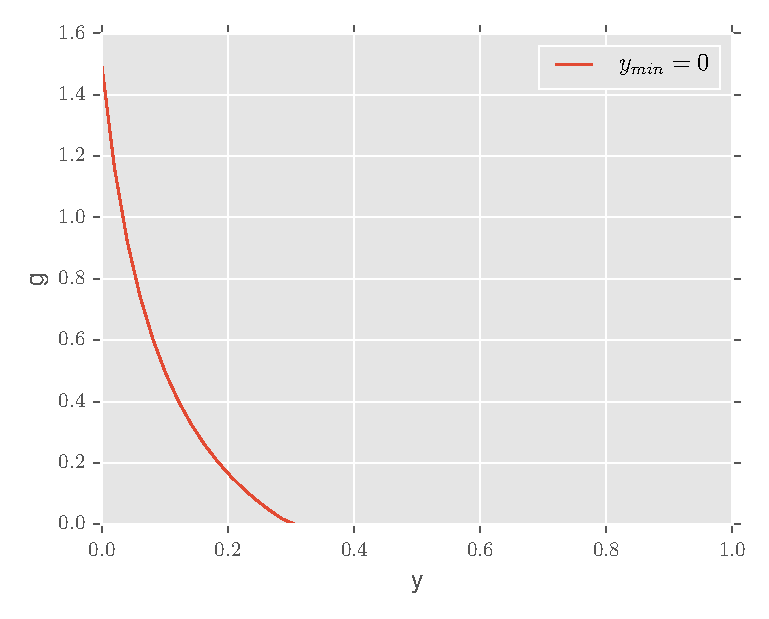
\includegraphics[keepaspectratio, width=4in]{g_2.pdf}
    \end{center}
  \vspace{-.2in} % corrects bad spacing
  \caption{\label{fig:g-2} Plot of $g(y)$ for \textit{Bottom Recession Process}.}
\end{figure}


\subsection*{Numerical Modeling}\label{sec:numerical-modeling}

We chose to model the parametric surface functions $x, y$ with discrete Fourier series. This is because spectral methods using the DFT will maintain the smoothness of the surface much better than a local approximation of the surface using finite differences which only acts locally at points. The DFT and surface derivatives can be calculated quickly using the Fast Fourier Transform (refer to Appendix \ref{sec:dft} for more details).

To integrate Equation \ref{eq:erosion-diff-eq}, we sample the surface at parameter values $S_n = 2 \pi \, \frac{n}{N} \; , \; n = 0, \dotsc, N-1$, which gives us a matrix of initial evaluation points

\begin{align*} 
  X_0 =& \bvec{r}\paren{0, S}\\
  =& \begin{bmatrix}
    x(0, S_1)& y(0, S_1)\\
    \vdots& \vdots\\
    x(0, S_N)& y(0, S_N)\\ 
  \end{bmatrix}
\end{align*}

\textbf{Note:} When refering to vectors and matrices in our numerical models, we will use uppercase letters to distinguish them from continuous functions.

Forward time integration of Equation \ref{eq:erosion-diff-eq} can then be implemented with standard ODE time stepping integration methods. In this paper, we used SciPy's {\tt odeint} method for integrating Equation \ref{eq:erosion-diff-eq}.

\subsection*{Point Collision Problems}

Unfortunately, the simplicity gained from modeling the surface with a Fourier series is soon lost when we start time stepping. As can be seen in Figure \ref{fig:remove-lowest-blob-bad}, the surface forms loops as time is increased (a physical impossibility).

\begin{figure}[H]
    \begin{center}
      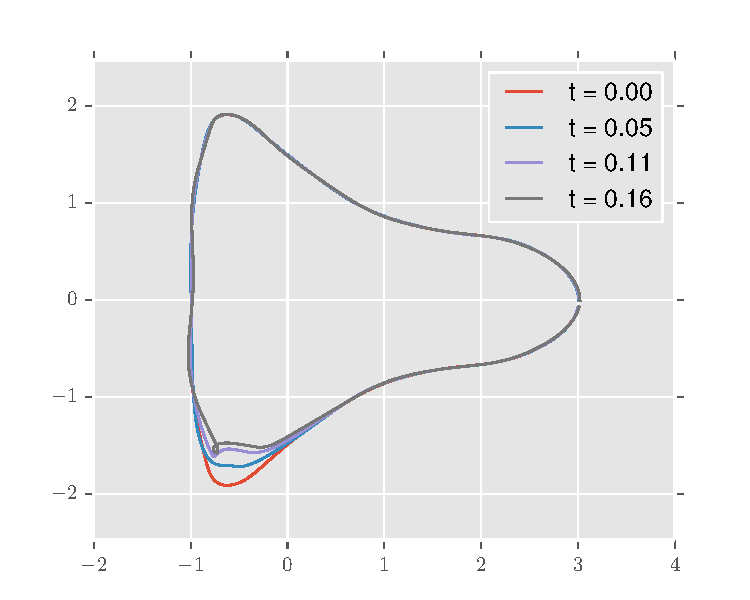
\includegraphics[keepaspectratio, width=4in]{remove_lowest_blob_bad.pdf}
    \end{center}
  \vspace{-.2in} % corrects bad spacing
  \caption{Time integration of \ref{eq:erosion-diff-eq} showing loop artifact.\label{fig:remove-lowest-blob-bad}}
\end{figure}

To investigate why these loop artifacts occur, we will show a zoomed in portion of the same figure, with the evaluation points shown. 

\begin{figure}[H]
    \begin{center}
      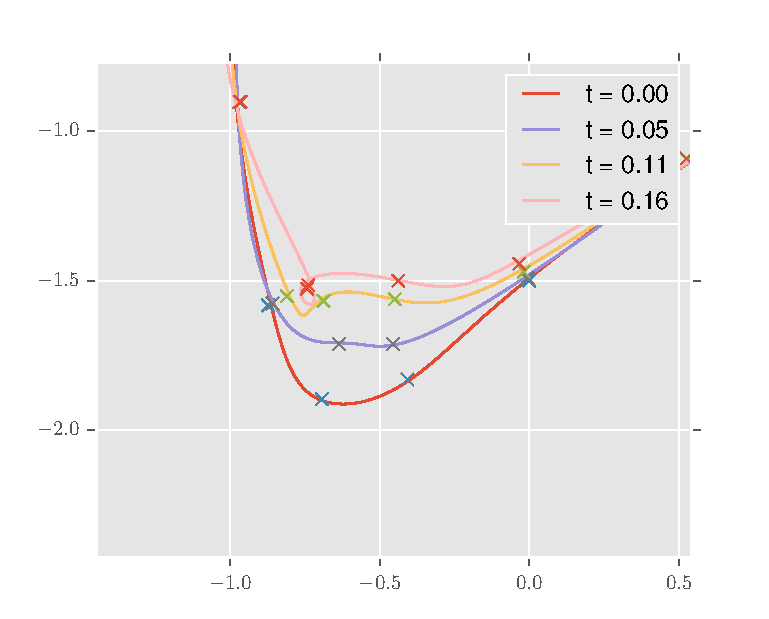
\includegraphics[keepaspectratio, width=4in]{remove_lowest_blob_bad_zoom.pdf}
    \end{center}
  \vspace{-.2in} % corrects bad spacing
  \caption{Expanded view of loop artifact.\label{fig:remove-lowest-blog-bad-zoom}}
\end{figure}

Looking closely, it can be seen that areas of high curvature form when evaluation points get close to each other, and this eventually leads to surface looping. Our guess is that this occurs because we are using discrete time stepping, so there are errors in the approximation of the shape's change with time. This is fine when the evaluation points are far from each other, but when they get close to each other, the errors become significant and affect the direction of the surface unit normal vectors. The folding causes unit normal vectors of nearby points to point at each other and which subsequently causes the points to cross over each other.

\subsection*{Redistributing Points}

A seemingly obvious way to fix this problem would be to resample to get a set of evenly spaced evaluation points on the surface. This wouldn't be too difficult of a task, since we can integrate and sample at any point on the surface via the FFT. Unfortunately, if we pick points on the surface at arbitrary values of $s$, we lose spectral accuracy, because we are now sampling at unevenly spaced values of our parameter $s$, which we will call $\tilde{S}$. The Discrete Fourier transform assumes that our points are sampled at evenly spaced values of $s$. Although we are working with the discrete Fourier transform, we need to return to the continuous equations to understand the problem. Redistribution in the continuous sense is a parameter transformation

\[ 
  \tilde{s} = h(s)
\]

with the condition of even spacing being

\[
  \norm{\frac{\partial \bvec{r}(s)}{\partial \tilde{s}}} = constant
\]

Our shape function now becomes

\[ \tilde{x}(s) = (x \circ h)(s) \]

There is absolutely no guarentee that the Fourier series of this composite function will decay at a reasonable rate, so using the DFT with our chosen resolution N could very poorly capture the surface shape. The method is not withough hope, since the technique of parameter transformation is utilized extensively in spectral methods such as the transformation $h(s) = \cos(s)$ used for Chebyshev spectral methods to cluster evaluation points near the endpoints of the domain. We need to find a way to generate a parameter transformation $h(s)$ where $(x \circ h)(s)$ has a rapidly decaying Fourier series.

\subsection*{Continuous Redistribution}

If we fix a time $t = t_1$, then we can define a differential equation that will allow us to redistribute the points and ensure that our redistributed points will still have a rapidly decaying Fourier series.

Physically $\dot{\bvec{r}}(t_1, s)$ is the surface tangent vector, and $\ddot{\bvec{r}}(t_1, s)$ is the rate of change of this surface tangent vector with respect to $s$. More importantly though, $\norm{\dot{\bvec{r}}(t_1, s)}$ is inversely proportional to the density of evaluation points on the surface at $s$. We would like to shift the evaluation points away from denser areas, thus we need move the evaluation points in the direction of larger $\norm{\dot{\bvec{r}}(t_1, s)}$, which is the projection of $\ddot{\bvec{r}}(t_1, s)$ onto the surface tangent vector.

\begin{equation}
  a_t(t, s) = \ddot{\bvec{r}}(t, s) \cdot \dot{\bvec{r}}(t, s)
\end{equation}


We can now set up a differential equation for this redistribution process.

\begin{equation}
  \label{eq:redist-diff-eq}
  \frac{\partial \bvec{r}(t_1, \tilde{s}(t'))}{\partial t'} = a_t(t_1, \tilde{s}(t')) \frac{\dot{\bvec{r}}(t_1, \tilde{s}(t'))}{\norm{\dot{\bvec{r}}(t_1, \tilde{s}(t'))}} \; , \quad \tilde{s}(0) = s
\end{equation}

To simplify the numerical computation, we can combine Equations \ref{eq:erosion-diff-eq} and \ref{eq:redist-diff-eq} to get a single ODE

\begin{equation}
  \frac{\partial (\bvec{r}(t, s))}{\partial t} = g(t, s) \; \bhat{n}(t, s) + a_t(t, s) \; \frac{\dot{\bvec{r}}(t_1, s)}{\norm{\dot{\bvec{r}}(t_1, s)}}
\end{equation}

As can be seen in Figure \ref{fig:remove-points-blob-good}, this modification dramatically improves our algorithm.

\begin{figure}[H]
    \begin{center}
      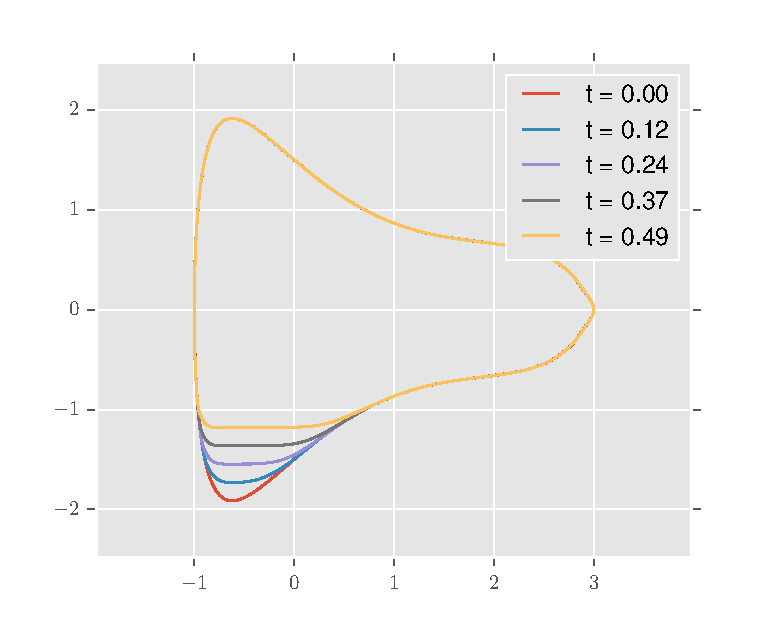
\includegraphics[keepaspectratio, width=4in]{remove_points_blob_good.pdf}
    \end{center}
  \vspace{-.2in} % corrects bad spacing
  \caption{\label{fig:remove-points-blob-good}\textit{Bottom recession process} simulation with point redistribution.}
\end{figure}

If we plot the evaluation points (Figure \ref{fig:remove-points-blob-good-points}), it can be seen that the points nicely redistribute themselves as time increases to stay evenly spaced on the surface.

\begin{figure}[H]
    \begin{center}
      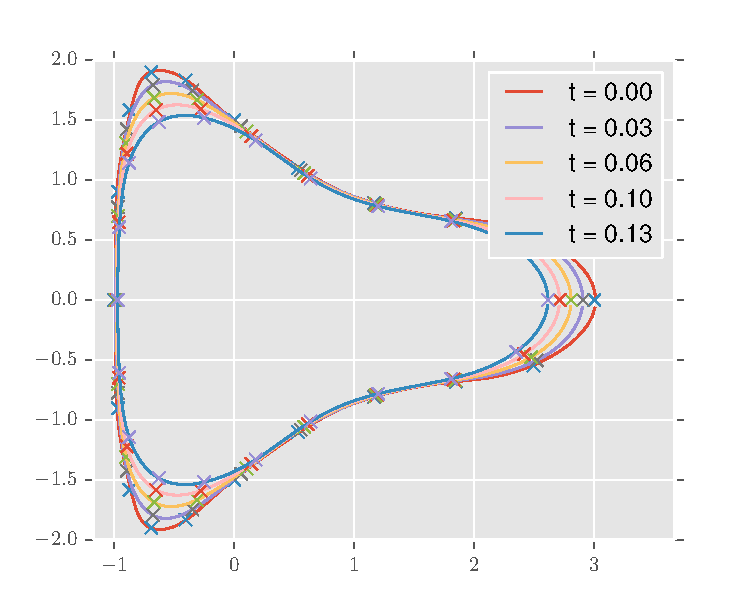
\includegraphics[keepaspectratio, width=4in]{remove_points_blob_good_points.pdf}
    \end{center}
  \vspace{-.2in} % corrects bad spacing
  \caption{\label{fig:remove-points-blob-good-points}\textit{Smoothing process} simulation with evaluation points shown.}
\end{figure}

\subsection*{Higher dimensions}

A next logical step would be to generalize the algorithm to a 2-dimensional surface that would be parameterized by $s_1, s_2 \in [0, 2\pi)$. Much of the algorithm would be similar, except that we would need to use the 2-dimensional discrete Fourier transform (refer to Appendix \ref{sec:dft}).

The surface normal vector equation for a surface in 3-dimensional space is the following

\[
  \bvec{n}(t, s_1, s_2) = \frac{\partial \bvec{r}(t, s_1, s_2)}{\partial s_1} \times \frac{\partial \bvec{r}(t, s_1, s_2)}{\partial s_2} 
\]

Curvature $\kappa$ could be generalized to mean curvature $H$

\begin{align*}
  H(t, s_1, s_2)& = \frac{\nabla \cdot \bvec{n}(t, s_1, s_2)}{2}\\
  &= \frac{1}{2} \paren{\frac{\partial \bvec{n}_1(t, s_1, s_2)}{\partial s_1} + \frac{\partial \bvec{n}_2(t, s_1, s_2)}{\partial s_2}}
\end{align*}

Avoiding singularities when mapping the 2-dimensional surface to an N x N array would likely be difficult, but the mapping only needs to be used to sample the initial points on the object, and the redistribution algorithm can be oblivious to the mapping.

